%-----------------------------------------------------------------
% Rodrigo Chang, 2019
% Banco de Guatemala
% Programa de Estudios Superiores 2019-2020
% Diapositivas del curso "Programación I"
%
% Descargo de responsabilidad.
%   El contenido de este documento es responsabilidad exclusiva de
% su(s) autores. Cualquier opinión expresada no necesariamente
% representa la postura institucional del Banco de Guatemala. 
% 
% Contenido.
%   El contenido de estas diapositivas está construido a partir de 
% modificaciones al material provisto por Ana Bell, Eric Grimson y 
% John Guttag para el curso 6.0001 Introduction to Computer Science 
% and Programming in Python, otoño 2016, Massachusetts Institute of 
% Technology: MIT OpenCourseWare, https://ocw.mit.edu
%
% Licencia: 
% Creative Commons BY-NC-SA
% https://creativecommons.org/licenses/by-nc-sa/4.0/.
%
% Formato. 
%   El formato utilizado para la elaboración de este documento 
% ha sido modificado a partir del repositorio: 
%       https://github.com/rinnert/statlearning-python-pwf
%
% Kurt Rinnert, 2019
%   Copying and distribution of this file, with or without 
% modification, are permitted in any medium without royalty provided 
% the copyright notice and this notice are preserved. This file is 
% offered as-is, without any warranty.
%
%-----------------------------------------------------------------
\documentclass[mathserif]{beamer}
% Para configurar las diapositivas en relación 16:9, 
% agregar la opción aspectratio=169

% Título de la presentación y tópicos a tratar
\usepackage{arev, arevmath}
\usepackage[scaled]{cabin}
%\usepackage[T1]{fontenc}
\usepackage[super]{nth}
\usepackage{pifont}
\usepackage{wasysym}
\usepackage{tabularx}
\usepackage{array}
\usepackage{booktabs}
\usepackage{boldline}
\usepackage{colortbl}
\usepackage{amsmath}
\usepackage{bm}
\usepackage{tcolorbox}
\usepackage{adjustbox}
\usepackage{minibox}
\usepackage{makecell}
\usepackage{adjustbox}
\usepackage{textcomp}
\usepackage[absolute,overlay]{textpos}
\setlength{\TPHorizModule}{1mm}%
\setlength{\TPVertModule}{1mm}%
\tcbuselibrary{skins}
\usepackage{graphicx}
\usepackage[spanish, es-tabla]{babel}
\usepackage[utf8]{inputenc}
\usepackage{csquotes}

\usepackage{comment}
\usepackage{svg}

\usepackage{verbatim}
\usepackage{pdfpages}

% Columnas múltiples
\usepackage{multicol}

% -------------------------------------------
%	LISTINGS
% -------------------------------------------
% Paquetes necesarios para los códigos
\usepackage{listings}
\usepackage{color}
% Configuración de listings (pendiente)
%\input{conf/listingStyles}
% Redefinición de titulos de caption
\renewcommand\lstlistingname{\textbf{Código}}
\renewcommand\lstlistlistingname{Códigos}

% Definición de colores para Python (Jupyter notebooks)
\definecolor{python_keyword_color}{RGB}{0, 128, 0}
\definecolor{python_string_color}{RGB}{186, 34, 34}
\definecolor{python_comment_color}{RGB}{1, 121, 121}
\definecolor{frame_numbers_color}{rgb}{0.5,0.5,0.5}
\definecolor{python_identifier_color}{RGB}{0,0,0}
\definecolor{jupyter_background}{RGB}{247, 247, 247}
\definecolor{jupyter_frame}{RGB}{207, 207, 207}

% Definicion de estilo para Python
\lstdefinestyle{custom_python}{
	language=python,			% the language of the code
	backgroundcolor=\color{jupyter_background}, 
	% the size of the fonts that are used for the code
	basicstyle=\linespread{1}\small\ttfamily,	
	% Configuración de colores
	commentstyle=\color{python_comment_color},	% comment style
	identifierstyle=\color{python_identifier_color},
	keywordstyle=\mdseries\color{python_keyword_color},	% keyword style
	numberstyle=\tiny\color{frame_numbers_color},	
	stringstyle=\color{python_string_color}, % string literal style 
	captionpos=t,				% sets the caption-position to bottom
	breakatwhitespace=false,	% sets if automatic breaks should only happen at whitespace
	breaklines=true,			% sets automatic line breaking
	morekeywords={},			% if you want to add more keywords to the set
	deletekeywords={eps},		% delete keywords from the given language
	escapeinside={\%*}{*)},		% if you want to add LaTeX within your code
	framesep=3pt,
	keepspaces=true,			% keeps spaces in text,       
	numbers=none, 	% (none, left, right)
	numbersep=5pt,	% how far the line-numbers are from the code
	% if not set, the frame-color may be changed on line-breaks within not-black text (e.g. comments (green here))
	rulecolor=\color{jupyter_frame}, 
	% show spaces everywhere adding particular underscores; it overrides 'showstringspaces'
	showspaces=false,                
	% underline spaces within strings only
	showstringspaces=false,          
	% show tabs within strings adding particular underscores
	showtabs=false,                  
	stepnumber=0,	% the step between two line-numbers      
	% sets default tabsize to 2 spaces
	tabsize=2,                       
	% lets you use non-ASCII characters; for 8-bits encodings only, does not work with UTF-8
	extendedchars=true,      
	% Support additional characters            
	literate=
  {á}{{\'a}}1 {é}{{\'e}}1 {í}{{\'i}}1 {ó}{{\'o}}1 {ú}{{\'u}}1
  {Á}{{\'A}}1 {É}{{\'E}}1 {Í}{{\'I}}1 {Ó}{{\'O}}1 {Ú}{{\'U}}1
  {à}{{\`a}}1 {è}{{\`e}}1 {ì}{{\`i}}1 {ò}{{\`o}}1 {ù}{{\`u}}1
  {À}{{\`A}}1 {È}{{\'E}}1 {Ì}{{\`I}}1 {Ò}{{\`O}}1 {Ù}{{\`U}}1
  {ä}{{\"a}}1 {ë}{{\"e}}1 {ï}{{\"i}}1 {ö}{{\"o}}1 {ü}{{\"u}}1
  {Ä}{{\"A}}1 {Ë}{{\"E}}1 {Ï}{{\"I}}1 {Ö}{{\"O}}1 {Ü}{{\"U}}1
  {â}{{\^a}}1 {ê}{{\^e}}1 {î}{{\^i}}1 {ô}{{\^o}}1 {û}{{\^u}}1
  {Â}{{\^A}}1 {Ê}{{\^E}}1 {Î}{{\^I}}1 {Ô}{{\^O}}1 {Û}{{\^U}}1
  {œ}{{\oe}}1 {Œ}{{\OE}}1 {æ}{{\ae}}1 {Æ}{{\AE}}1 {ß}{{\ss}}1
  {ű}{{\H{u}}}1 {Ű}{{\H{U}}}1 {ő}{{\H{o}}}1 {Ő}{{\H{O}}}1
  {ç}{{\c c}}1 {Ç}{{\c C}}1 {ø}{{\o}}1 {å}{{\r a}}1 {Å}{{\r A}}1
  {€}{{\EUR}}1 {£}{{\pounds}}1,   
}

% Configurar el listing para el documento actual
\lstset{
	style = custom_python, 
	frame = single
}

% -------------------------------------------
%	OTRAS CONFIGURACIONES
% -------------------------------------------
\makeatletter
\newcommand{\antsize}{\@setfontsize{\antsize}{4pt}{4pt}}
\makeatother
\newcommand{\at}{\makeatletter @\makeatother}

\newcommand{\cmark}{\ding{51}}%
\newcommand{\bottomline}[1]{\vskip0pt plus 1fill{\alert{#1}\phantom{g}\vskip 1.0mm}}

% Rutas para las imágenes
%\graphicspath{{figs/}{figs/common/}}

% Separación de filas en las tablas más amplia
\renewcommand{\arraystretch}{1.2}


% -------------------------------------------
%	ESTILO DE LA PRESENTACIÓN
% -------------------------------------------

\mode<presentation>%
{
	\usetheme{default}
	%\usetheme[width=2.5cm]{PaloAlto}
	\usecolortheme{dove}
	\useoutertheme{infolines}
	% oder auch nicht

	% BANGUAT Colors
	\definecolor{BANGUATblue}{RGB}{37,86,162} % 0x255682
	\definecolor{BANGUATorange}{RGB}{255,130,0} % 0xff8200
	\definecolor{BANGUATgreen}{RGB}{0,100,0}
	\definecolor{BANGUATdark}{RGB}{80,80,80} % 0x505050
	\definecolor{BANGUATlight}{RGB}{120,120,120}
	\definecolor{BANGUATbrown}{RGB}{178,91,0}

	\definecolor{codebg}{rgb}{0.95,0.95,0.95}

	% Color theme
	\setbeamercolor{alerted text}{fg=BANGUATorange}
	\setbeamercolor{frametitle}{fg=BANGUATblue}
	\setbeamercolor{title}{fg=BANGUATblue}
	\setbeamercolor{subtitle}{fg=BANGUATorange}
	\setbeamercolor{normal text}{fg=BANGUATdark}
	\setbeamercolor{author in foot}{fg=BANGUATblue}
	\setbeamercolor{item}{fg=BANGUATblue}
	\setbeamercolor{footline}{fg=BANGUATblue}
	%\setbeamercolor{item projected}{bg=BANGUATorange}
	%\setbeamercolor{item projected}{fg=white}

	\setbeamertemplate{headline}
	{}
	\setbeamertemplate{frametitle}
	{
		%\textbf{{\insertframetitle\phantom{g}}}\\
		%\textbf{\insertframetitle\phantom{g}}\\
		\textbf{\underline{\insertframetitle\phantom{g}}}\\
		%\textbf{\underline{\insertframetitle}}\\
		\vskip 1.0mm
		%{\color{UOLgold}\hrule height 2pt}
		%\par
	}
	\addtobeamertemplate{frametitle}{}{\vspace{-1em}}
	\setbeamertemplate{footline}{
		{%
			\textbf{ \hskip 3.0mm\insertshorttitle\phantom{.}---\phantom{.}\insertshortinstitute\hfill\insertframenumber\,/\,\inserttotalframenumber\hskip 3.0mm} 
		}
	}

	\setbeamertemplate{navigation symbols}{}%remove navigation symbols
	\setbeamertemplate{itemize items}[circle]
	\setbeamertemplate{enumerate items}[fg=BANGUATblue]
	\setbeamercolor{itemize items}{fg=BANGUATblue}
	\setbeamercolor{sidebar}{bg=BANGUATblue}
	\setbeamercolor{title in sidebar}{fg=BANGUATorange}
	\setbeamercolor{author in sidebar}{fg=BANGUATorange}
	\setbeamercolor{section in sidebar}{fg=BANGUATorange}
}



% -------------------------------------------
%	CONFIGURACIÓN DE DIAPOSITIVA DE TÍTULO
% -------------------------------------------

% Título del curso
\title[Programación I]{\textbf{%
Introducción a las ciencias de la computación\\%
{\it y programación en Python}}\\%
%\href{https://ocw.mit.edu/courses/electrical-engineering-and-computer-science/6-0001-introduction-to-computer-science-and-programming-in-python-fall-2016/}{\tiny\it Basado en el curso ``Introduction to Computer Science and Programming in Python'' por Ana Bell, Eric Grimson, y John Guttag.}%
\vspace{3em}%
}
%\vspace{-2.5cm}{}

% Autor y correo electrónico
\author{\href{mailto:?to=Rodrigo Chang <rrcp@banguat.gob.gt>&subject=PES Programación I}{Rodrigo Chang}}

% Información del instituto
\institute[\href{https://www.banguat.gob.gt/}{Banco de Guatemala}]%
{\color{BANGUATblue} \bfseries \href{https://www.banguat.gob.gt/}{Banco de Guatemala}\\%
\vspace{3mm}%

\includegraphics[width=0.13\textwidth]{figs/common/logo-banguat.png}}

% Sin fecha en particular
\date{}

% Información de licencias y copyright
\titlegraphic{
	 %\texorpdfstring{\vspace{-3cm}}{}
	 \vspace{-1.5cm}
	 \begin{minipage}[b][1cm][b]{0.25\textwidth}%
	    \color{BANGUATlight}\antsize
		%Copyright \textcopyright~2019\\
		\href{mailto:?to=Rodrigo Chang <rrcp@banguat.gob.gt>&subject=PES Programación I}{Rodrigo Chang <rrcp@banguat.gob.gt>}\\
		Este material está construido a partir de modificaciones al material provisto por Ana Bell, Eric Grimson y John Guttag para el curso \textit{6.0001 Introduction to Computer Science and Programming in Python}, otoño 2016, Massachusetts Institute of Technology: MIT OpenCourseWare, \href{https://ocw.mit.edu}{https://ocw.mit.edu}. Licencia: \href{https://creativecommons.org/licenses/by-nc-sa/4.0/}{Creative Commons BY-NC-SA}.
		
		%Copying and distribution of this file, with or without modification, are permitted in any medium without royalty provided the copyright notice and this notice are preserved.  This file is offered as-is, without any warranty.


		%Some of the figures in this presentation are taken from ``An Introduction to Statistical Learning, with applications in R''  (Springer, 2013) with permission from the authors: G. James, D. Witten,  T. Hastie and R. Tibshirani 
	 \end{minipage}%
	 \hspace{9cm}
}

% Restar uno al contador
\addtocounter{framenumber}{-1}

% Cajas de colores
\newcommand{\tabboxset}{\tcbset{enhanced, nobeforeafter, boxrule=0pt, boxsep=0pt, colback=codebg, colframe=codebg, coltext=BANGUATdark, rounded corners, arc=4pt, fonttitle={\bfseries\tiny}}}
\newcommand{\codeboxset}{\tcbset{enhanced, nobeforeafter, boxrule=0pt, boxsep=0pt, colback=codebg, colframe=codebg, coltext=BANGUATdark, rounded corners, arc=4pt, fonttitle={\bfseries\tiny}}}

% Comandos útiles
\newcommand{\orange}{\color{BANGUATorange}}
\newcommand{\blue}{\color{BANGUATblue}}
\newcommand{\dark}{\color{BANGUATdark}}
\newcommand{\R}{\mathbb{R}}
\newcommand{\dat}[1]{{\footnotesize\tt\orange #1}}
\newcommand{\mdat}[1]{\text{\dat{#1}}}
\newcommand{\val}[1]{{\footnotesize\tt\blue #1}}
\newcommand{\mval}[1]{\text{\val{#1}}}
\newcommand{\e}[1]{\emph{#1}}
\newcommand{\bh}{\hat{\beta}}
\newcommand{\h}{\hat}
\newcommand{\bl}{\bottomline}


\makeatletter
\newcommand{\includegraphicsdpi}[3]{%
	\pdfimageresolution=#1%
	\includegraphics[#2]{#3}%
	\pdfimageresolution=72%
}

\newcommand{\Quote}[2]{%
	\begin{center} 
		\begin{minipage}{0.7\textwidth} 
			\hrule
			\vskip 3mm
			\emph{{\color{BANGUATblue} ``#1''}\\
			{\color{BANGUATorange} --- #2}}
			\vskip 3mm
			\hrule
			\vskip 2mm
		\end{minipage}
	\end{center}
}

% Texto centrado en la diapositiva, quizás para el abstract o para indicar abajo de un quote
\newenvironment{blurb}%
	{\begin{center}\begin{minipage}{0.6\textwidth}\footnotesize}
	{\end{minipage}\end{center}}

% Environment para códigos o algoritmos. Parecido a un bottomline, se puede utilizar para dar definiciones o enfatizar en algún concepto
\newenvironment{cpage}%
	{\begin{center}\begin{minipage}{0.75\textwidth}}
	{\end{minipage}\end{center}}

% Bloque (similar a un pop-up) de alerta para indicar resultados en tablas, definiciones, fórmulas, etc.
% Primer argumento es el tamaño 
% Segundo argumento es el título del bloque
\newenvironment{popblock}[2]%
	{\begin{center}\begin{minipage}{#1}\footnotesize
		\begin{tcolorbox}[colframe=codebg, colback=white, colupper=BANGUATdark, title={\normalsize\bfseries\blue #2}]}
	{\end{tcolorbox}\end{minipage}\end{center}}
\makeatother

% Incluir diapositivas en PDF
% 1 - Título de la diapositiva
% 2 - páginas del PDF a incluir
% 3 - ruta hacia el archivo PDF
\newcommand{\includeslides}[3]{%
{%
\setbeamercolor{background canvas}{bg=}%
\addtocounter{framenumber}{1}%
\includepdf[pages={#1}, link=true, pagecommand={%
\Large\blue\bfseries\underline{%
#3\phantom{g}}%
\vspace{-1em}%
\vskip 1.0mm}]{#2}%
}}
\subtitle{\bfseries%
  {Manejo de strings, \textit{guess and check}, métodos de aproximación}\\%
  %{\tiny\it Manejo de strings, \textit{guess and check}, métodos de aproximación}\\%
}

% Inicio del documento
\begin{document}
\frame[plain]{
	%\vskip 1.0mm
	\titlepage
	%\vskip 1.0mm
}
%-----------------------------------------------------------------
% Empieza el contenido de la presentación
%-----------------------------------------------------------------

\begin{frame}{Abstract}
	\Quote{Everybody should learn to program a computer, because it teaches you how to think}{Steve Jobs}
    
	\begin{blurb}
		Veremos un poco más acerca de la manipulación de cadenas de texto. 
		
		Hablaremos de los algoritmos \textit{guess and check}. 
		
		Conoceremos algunas aplicaciones de este tipo de algoritmos.
	\end{blurb}
\end{frame}

\section{Manipulación de cadenas de texto}

\begin{frame}[fragile]{Cadenas de texto}
    \begin{itemize}
        \item Tipo de datos {\blue no escalar} en Python. 
        
        \item Algunos operadores curiosos definidos: \lstinline|>, <, ==|.
        
        \item Podemos utilizar la función \lstinline|len()| para obtener el largo de la cadena.
\begin{lstlisting}
s = "abcde"
len(s) # devuelve 3
\end{lstlisting}
    \end{itemize}
\end{frame}

\begin{frame}[fragile]{Cadenas de texto}
    \begin{itemize}
        \item Los objetos de tipo \lstinline|str| poseen estructura. Esto nos permite {\blue\bfseries indexar} los caracteres que la conforman.
\begin{lstlisting}
s[0]  # -> devuelve "a"
s[1]  # -> devuelve "b"
s[2]  # -> devuelve "c"
s[3]  # -> fuera de límites, error
s[-1] # -> devuelve "c"
s[-2] # -> devuelve "b"
s[-3] # -> devuelve "a"
\end{lstlisting}
        
    \end{itemize}
\end{frame}

\begin{frame}[fragile]{\textit{Slicing}}
    \begin{itemize}
        \item Las cadenas se pueden ``partir'' utilizando \lstinline|[start:stop:step]|. 
        
        \item Si \lstinline|[start:stop]|, \lstinline|step = 1| por defecto.
        
        \item Se pueden {\blue omitir} números y dejar \lstinline|:|
    \end{itemize}
    
\begin{lstlisting}
s = "abcdefgh"
s[3:6]   # -> devuelve "def", s[3:6:1]
s[3:6:2] # -> devuelve "df"
s[::]    # -> devuelve "abcdefgh", s[0:len(s):1]
s[::-1]  # -> devuelve "hgfedbca", s[-1:-(len(s)+1):-1]
s[4:1:-2]# -> devuelve "ec"
\end{lstlisting}
\end{frame}


\begin{frame}[fragile]{Inmutabilidad}
    \begin{itemize}
        \item Las cadenas de texto son ``inmutables'' \lstinline|=| no pueden ser modificadas.
    \end{itemize}
    
\begin{lstlisting}
s = "hello"
s[0] = 'y'            # error
s = 'y' + s[1:len(s)] # redefinir
\end{lstlisting}

    \begin{figure}
        \centering
        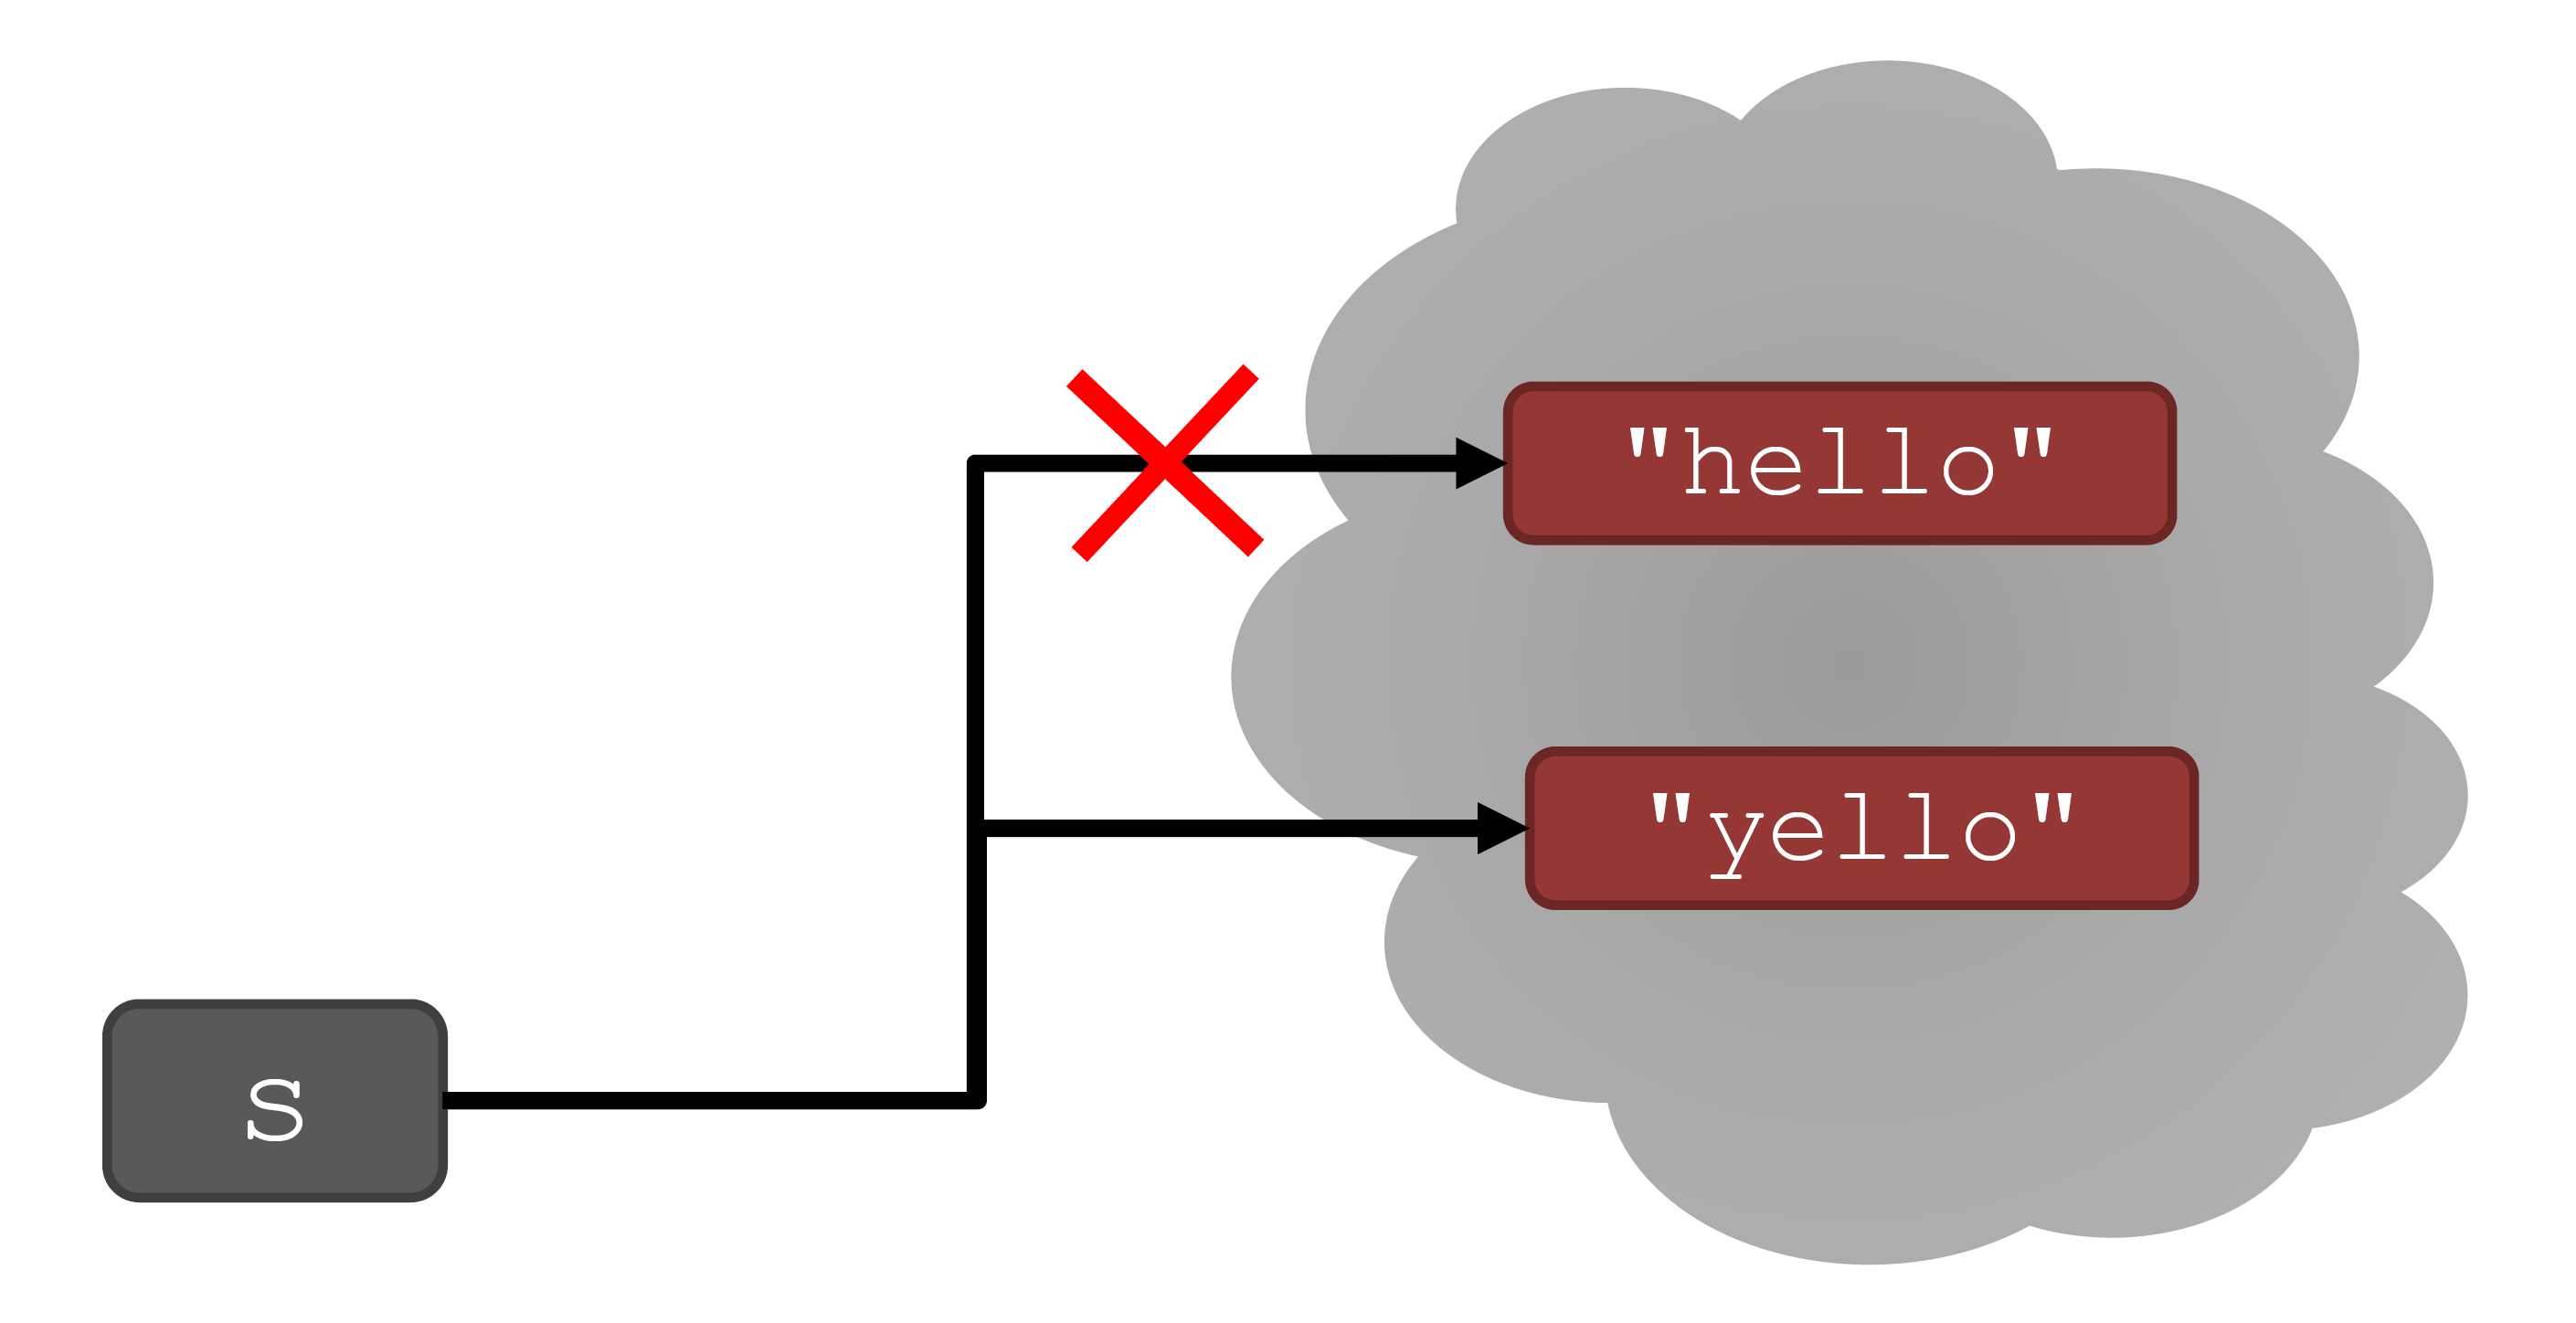
\includegraphics[width=0.5\textwidth]{figs/strings/inmutability-strings.png}
    \end{figure}
\end{frame}

\begin{frame}[fragile]{Recapitulación de \lstinline|for|}
    \begin{itemize}
        \item Previamente, aprendimos que \lstinline|for| trabaja en conjunto con la función \lstinline|range|.
\begin{lstlisting}
for var in range(4): 
    <expresiones>
    ...

for var in range(4, 10):
    <expresiones>
    ...
\end{lstlisting}

        \item Los ciclos \lstinline|for| pueden iterar sobre {\blue cualquier conjunto de valores}, ¡no solamente números!

    \end{itemize}
\end{frame}

\begin{frame}[fragile]{Cadenas de texto y ciclos}
    \begin{itemize}
        \item Los bloques de abajo son {\blue\bfseries equivalentes}.
        
    \end{itemize}
\begin{lstlisting}
s = "abcdefgh"

for index in range(len(s)):
    if s[index] == 'i' or s[index] == 'u':
        print("There is an i or u")

for char in s:
    if char == 'i' or char == 'u':
        print("There is an i or u")
\end{lstlisting}

    \bottomline{El último es más \textit{Pythónico}.}
\end{frame}

\begin{frame}[fragile]{Ejemplo: porristas robot}
\begin{lstlisting}
an_letters = "aefhilmnorsxAEFHILMNORSX"
word = input("I will cheer for you! Enter a word: ")
times = int(input("Enthusiasm level (1-10): "))

i = 0
while i < len(word):
   char = word[i]
   if char in an_letters:
       print("Give me an " + char + "! " + char)
   else:
       print("Give me a  " + char + "! " + char)
   i += 1
   
print("What does that spell?")
for i in range(times):
   print(word, "!!!")
\end{lstlisting}
\end{frame}

\begin{frame}[fragile]{Ejemplo: porristas robot}
\begin{lstlisting}
an_letters = "aefhilmnorsxAEFHILMNORSX"
word = input("I will cheer for you! Enter a word: ")
times = int(input("Enthusiasm level (1-10): "))

for char in word:
   if char in an_letters:
       print("Give me an " + char + "! " + char)
   else:
       print("Give me a  " + char + "! " + char)
       
   
print("What does that spell?")
for i in range(times):
   print(word, "!!!")
\end{lstlisting}
\end{frame}



\section{Guess and check}

\begin{frame}{\textit{Guess and check}}
    \begin{itemize}
        \item A este tipo de algoritmos se les conoce también como de {\bfseries\blue enumeración exhaustiva}. 
    \end{itemize}
    
    \begin{cpage}
    \begin{enumerate}
        \item Dado un problema.
        \item Podemos {\blue proponer/adivinar} una solución.
        \item Podemos {\blue verificar} que la solución es correcta.
        \item Repetimos 1,2 y 3 hasta encontrar la solución.
    \end{enumerate}
    \end{cpage}
\end{frame}

\begin{frame}[fragile]{Cubos perfectos}
    \begin{itemize}
        \item Veamos un ejemplo de {\bfseries\blue enumeración exhaustiva}.
        
\begin{lstlisting}
#cube = 27
##cube = 8120601

for guess in range(cube+1):
    if guess**3 == cube:
        print("Cube root of", cube, "is", guess)
\end{lstlisting}

        \item ¿Cómo podemos salir si encontramos la solución?
        \item ¿Qué pasa si \lstinline|cube| no tiene cubo perfecto o es negativo?
    \end{itemize}
\end{frame}

\begin{frame}[fragile]{Cubos perfectos}
    \begin{itemize}
        \item Veamos una posible solución
    \end{itemize}
\begin{lstlisting}
cube = 27
#cube = 8120601
for guess in range(abs(cube)+1):
   # passed all potential cube roots
   if guess**3 >= abs(cube):
       # no need to keep searching
       break
if guess**3 != abs(cube):
   print(cube, 'is not a perfect cube')
else:
   if cube < 0:
       guess = -guess
   print('Cube root of ' + str(cube) + ' is ' + str(guess))
\end{lstlisting}
\end{frame}

\section{Métodos de aproximación}

\begin{frame}[fragile]{Soluciones aproximadas}
    \begin{itemize}
        \item En ocasiones, basta con una solución lo {\blue\bfseries suficientemente buena}. 
        
        \begin{enumerate}
            \item Dado un problema.
            \item Emmpezamos con una solución y aumentamos por un {\blue pequeño valor}.
            \item Si \lstinline&|guess**3 - cube| >= epsilon &, seguimos probando. 
        \end{enumerate}
        
        \item Si aumentamos $\epsilon \Rightarrow$ {\blue menor precisión}.
        \item Si disminuimos $\epsilon \Rightarrow$ {\blue mayor lentitud}.
    \end{itemize} 
\end{frame}

\begin{frame}[fragile]{Raíz cúbica aproximada}
    \begin{itemize}
        \item Veamos el siguiente ejemplo.
    \end{itemize}
\begin{lstlisting}[numbers=left]
cube = 27

epsilon = 0.1
guess = 0.0
increment = 0.01
num_guesses = 0
# look for close enough answer and make sure
# didn't accidentally skip the close enough bound
while abs(guess**3 - cube) >= epsilon and guess <= cube:
   guess += increment
   num_guesses += 1
print('num_guesses =', num_guesses)
if abs(guess**3 - cube) >= epsilon:
   print('Failed on cube root of', cube)
else:
   print(guess, 'is close to the cube root of', cube)
\end{lstlisting}
\end{frame}

\begin{frame}[fragile]{Búsqueda por bisección}
    \begin{columns}
        \begin{column}{0.5\textwidth}
            \centering
            \includesvg[width=0.9\textwidth]{figs/strings/Bisection_method}
        \end{column}
        \begin{column}{0.5\textwidth}
            \begin{itemize}
                \item En cada iteración, seleccionamos una {\blue mitad} del intervalo.
                \item Solución candidata en el intervalo.
            \end{itemize}
        \end{column}
    \end{columns}
\end{frame}


\begin{frame}[fragile]{Raíces cúbicas}
\begin{lstlisting}
cube = 27

epsilon = 0.01
num_guesses, low = 0, 0
high = cube
guess = (high + low)/2.0

while abs(guess**3 - cube) >= epsilon:
   if guess**3 < cube:
       # look only in upper half search space
       low = guess
   else:
       # look only in lower half search space
       high = guess
   
   guess = (high + low)/2.0
   num_guesses += 1
print('num_guesses: ', num_guesses, 'raiz: ', guess)
\end{lstlisting}
\end{frame}

\begin{frame}[fragile]{Acerca de la convergencia}
    \begin{itemize}
        \item La solución candidata converge en un orden de $\log_2 N$ pasos.
        \item La {\blue búsqueda de bisección} funciona cuando la función varía {\blue monótonamente} de acuerdo a la entrada.
        
        \item El código anterior funciona solamente para cubos positivos mayores a $1$. ¿Por qué?
    \end{itemize}
    
    \bottomline{¿Cómo podemos modificar el código para que funcione con cubos negativos y positivos $< 1$?}
\end{frame}


%-----------------------------------------------------------------
% Termina el contenido de la presentación
%-----------------------------------------------------------------

\begin{comment}
\begin{frame}[fragile]{Búsqueda por bisección}
    \begin{columns}
        \begin{column}{0.5\textwidth}
        \end{column}
        \begin{column}{0.5\textwidth}
        \end{column}
    \end{columns}
\end{frame}

\begin{frame}[fragile]{}
    \begin{itemize}
        \item 
    \end{itemize}
\end{frame}
\end{comment}

\end{document}